%!TEX root = ../thesis.tex

% \subsection{QVF-DAGモデルの識別可能性}

本章では、前章で導入したQVF-DAGモデル\cite{Park2017-hw}が識別可能であることを証明する。
QVF-DAGモデルの識別可能性は
Park and Raskutti(2017)\cite{Park2017-hw}によって
過分散スコア(OverDispersion Score; ODS)を用いて初めて証明された。

過分散とは、ポアソン分布などの分散が期待値に依存する確率分布において、
期待される分散より標本分散の方が大きくなることである。
過分散が生じる原因の1つとして、サンプルの個体差などが挙げられる。
このような個体差などの効果を組み込んだ統計モデルに
一般化線形混合モデル(generalized linear mixed model; GLMM)がある\cite{2012-iq}。

統計的因果探索の文脈において最初に過分散を利用した例は、
Park and Raskutti(2015)\cite{Park2015-tj}のPoisson DAGモデルである。
Park and Raskutti(2015)\cite{Park2015-tj}では
Poisson DAGモデルの各頂点の条件付き分散が過分散であるかどうかを検定することによって、
識別可能性を証明している。
Park and Raskutti(2017)\cite{Park2017-hw}では、
Poisson DAGモデルにおける過分散が、
QVF-DAGモデルでも成立することを利用し、QVF-DAGモデルの識別可能性を証明している。
つまり、Park and Raskutti(2017)\cite{Park2017-hw}による
過分散スコアを用いたQVF-DAGモデルの識別可能性の証明は、
Park and Raskutti(2015)\cite{Park2015-tj}によるPoisson DAGモデルの識別可能性の証明の
自然な拡張であると言える。

Poisson DAGモデルの識別可能条件は、
Park and Park(2019)\cite{Park2019-qy}による
モーメント比スコア(Moment Ratio Score; MRS)を用いた証明も行われている。
モーメント比スコアを用いることによって、
識別可能条件が緩和され、DAGの推定精度やsample complexityも改善することが示されている\cite{Park2019-qy}。

そこで本論文では、Park and Park(2019)\cite{Park2019-qy}による
Poisson DAGモデルのモーメント比スコアを拡張することで、
QVF-DAGモデルの識別可能性を証明する。
そうすることで、従来の識別可能条件\cite{Park2017-hw}を緩和することや、
DAGの推定精度が向上することが期待される。

まず初めに、QVF-DAGモデルにおけるモーメント(積率)について
以下のような関係性が成立していることを示し、識別可能性の証明に利用する。

\begin{prop} \label{prop:MRS}
  リンク関数$(g_j(X_{Pa(j)}))_{j \in V}$が非退化であるQVF-DAGモデル~\eqref{QVF}において、
  任意の頂点$j \in V$、任意の集合$S_j \subset \mathit{Nd}(j)$に関して、
  以下のモーメント関係が成立する。
  \begin{equation}
    \frac{E(X_j^2)}
    {E \left[ \beta_0 E(X_j | X_{S_j}) + (\beta_1 + 1)E(X_j | X_{S_j})^2 \right]}
    \geq 1
    \label{eq:MRS}
  \end{equation}
  同様に、
  \begin{equation}
    E(\mathrm{Var}( E(X_j | X_{Pa(j)}) | X_{S_j} )) \geq 0
  \end{equation}
  等号成立は、$S_j$が頂点$j$の親変数すべてを含むとき($Pa(j)\subset S_j$)である。
\end{prop}

\begin{proof}
  分散とモーメントの関係性と、2次分散関数性の定義を利用すると、
  2次分散関数性を満たす確率変数$X$のモーメントについて、以下の関係性が成り立つ。
  \begin{alignat*}{2}
    \mathrm{Var}(X) &= E(X^2) - E(X)^2 & \qquad & \text{分散の公式より} \\
                    &= \beta_0 E(X) + \beta_1 E(X)^2 && \text{2次分散関数性の定義より}
  \end{alignat*}
  よって、
  \begin{equation*}
    E(X^2) = \beta_0 E(X) + (\beta_1 + 1) E(X)^2
  \end{equation*}

  ここで、記号の簡単のために、関数$f(\mu) = \beta_0 \mu + (\beta_1 + 1)\mu^2$を定義する。
  すると、任意の頂点$j \in V$、任意の空でない集合$S_j \subset \mathit{Nd}(j)$について、
  以下のように書ける。
  \begin{equation}
    \begin{split}
      E(X_j^2 | S_j) &= E(E(X_j^2 | X_{Pa(j)}) | S_j) \\
                     &= E(f(E(X_j | X_{Pa(j)})) | S_j)
      \label{moment_related}
    \end{split}
  \end{equation}

  イェンセンの不等式と関数$f(\cdot)$が凸であることを利用すると、以下が導ける。
  \begin{equation}
    \begin{split}
      E(f(E(X_j | X_{Pa(j)})) | S_j) & \geq
      f(E(E(X_j | X_{Pa(j)}) | S_j)) \\
      &= f(E(X_j | S_j))
      \label{Jensen}
    \end{split}
  \end{equation}

  ここで、モデルの定義より、$E(X_j | X_{Pa(j)}) = g_j(X_{Pa(j)})$であり、
  関数$g_j(\cdot)$は非退化であることを利用すると、
  等号は$S_j$が頂点$j$の親変数すべてを含むとき
  ($Pa(j) \subset S_j \subset \mathit{Nd}(j)$)のみ成立する。

  式~\eqref{moment_related}と式~\eqref{Jensen}を整理すると、
  \begin{equation*}
    \begin{split}
      E(X_j^2 | S_j) &- f(E(X_j | S_j)) \geq 0 \\
      E(X_j^2 | S_j) &- \bigl( \beta_0 E(X_j | S_j) +
      (\beta_1 + 1) E(X_j | S_j)^2 \bigl) \geq 0
    \end{split}
  \end{equation*}
  となり、
  さらに期待値を取ることで、
  \begin{equation}
    E(X_j^2) - E\bigl(\beta_0 E(X_j | S_j) + (\beta_1 + 1) E(X_j | S_j)^2 \bigl) \geq 0
    \label{proposition_1}
  \end{equation}
  が得られる。 よって、以下が成り立つ。
  \begin{equation}
    \frac{E(X_j^2)}
    {E\bigl( \beta_0 E(X_j | S_j) + (\beta_1 + 1) E(X_j | S_j)^2 \bigl)}
    \geq 1
    \label{proposition_2}
  \end{equation}

  ここからは、$E(X_j^2) \geq E\bigl( \beta_0 E(X_j | S_j) +
  (\beta_1 + 1) E(X_j | S_j)^2 \bigl)$ が、
  $E(\mathrm{Var}( E(X_j | X_{Pa(j)}) | X_{S_j} )) \geq 0$と
  同値であることを証明する。
  まず、分散の公式より以下のように書ける。
  \begin{equation}
    \label{variance}
    E(\mathrm{Var}(X_j | S_j))
     = E(E(\mathrm{Var}(X_j | X_{Pa(j)}) | S_j)) + E(\mathrm{Var}(E(X_j | X_{Pa(j)}) | S_j))
  \end{equation}
  ここで、モデルの定義~\eqref{QVF}を式~\eqref{variance}の右辺の第1項目に代入すると、以下のように整理できる。
  \begin{align}
    E(E(\mathrm{Var}(X_j | X_{Pa(j)}) | S_j))
      &= E(E(\beta_0 E(X_j | X_{Pa(j)}) + \beta_1 E(X_j | X_{Pa(j)})^2 | S_j)) \notag \\
      &= E(E(\beta_0 E(X_j | X_{Pa(j)}) | S_j)) + E(E(\beta_1 E(X_j | X_{Pa(j)})^2 | S_j)) \notag \\
      &= \beta_0 E(X_j) + \beta_1 E(X_j)^2
      \label{organize}
  \end{align}
  さらに、式~\eqref{organize}を用いて式~\eqref{variance}を整理すると、以下のように書ける。
  \begin{equation}
    \label{variance_2}
    E(\mathrm{Var}(E(X_j | X_{Pa(j)}) | S_j))
     = E(\mathrm{Var}(X_j | S_j)) - \beta_0 E(X_j) - \beta_1 E(X_j)^2
  \end{equation}

  ここから式~\eqref{variance_2}の右辺を整理すると、以下のように書ける。
  ただし、最後の不等号は式~\eqref{proposition_1}より成立する。
  \begin{align*}
    E(&\mathrm{Var}(X_j | S_j)) - \beta_0 E(X_j) - \beta_1 E(X_j)^2 \\
     &= E(E(X_j^2 | S_j) - E(X_j | S_j)^2) - \beta_0 E(X_j) - \beta_1 E(X_j)^2 \\
     &= E(E(X_j^2 | S_j)) - E(E(X_j | S_j)^2) - E(\beta_0 E(X_j | S_j)) - E(\beta_1 E(X_j | S_j)^2) \\
     &= E(X_j) - E(\beta_0 E(X_j | S_j) + (\beta_1 + 1) E(X_j | S_j)^2) \\
     & \geq 0
  \end{align*}

  よって、式~\eqref{eq:MRS}は、
  $E(\mathrm{Var}( E(X_j | X_{Pa(j)}) | X_{S_j} )) \geq 0$
  と同値である。
  \qed

\end{proof}

ここからは、命題\ref{prop:MRS}が
QVF-DAGモデルの識別可能性に利用できることを直感的に理解するために、
各頂点の親変数による条件付き確率分布がポアソン分布である
2変数DAGモデルを例にその識別可能性を証明する。
そこで、図\ref{fig:ex_bivariate}のようなDAGモデルを考える。

\begin{itemize}
  \item $G_1 \colon X_1 \sim \mathrm{Poisson}(\lambda_1),
         \quad X_2 \sim \mathrm{Poisson}(\lambda_2) \quad$ ただし、$X_1$と$X_2$は独立

  \item $G_2 \colon X_1 \sim \mathrm{Poisson}(\lambda_1),
         \quad X_2|X_1 \sim \mathrm{Poisson}(g_2(X_1))$

  \item $G_3 \colon X_2 \sim \mathrm{Poisson}(\lambda_2),
         \quad X_1|X_2 \sim \mathrm{Poisson}(g_1(X_2))$

  ただし、$g_1$と$g_2$は非退化な任意の関数である。
  $(g_1, g_2 \colon \mathbb{N} \cup \{ 0 \} \rightarrow \mathbb{R}^+)$
\end{itemize}

\begin{figure}[h]
  \centering
  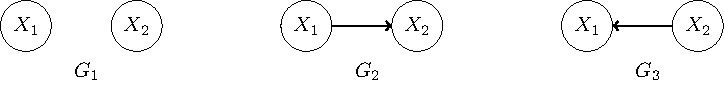
\includegraphics{./picture/bivariate.pdf}
  \caption{2変数のPoisson-DAGモデル}
  \label{fig:ex_bivariate}
\end{figure}

命題\ref{prop:MRS}より、$G_1$におけるすべての頂点$j \in \{ 1,2 \}$について、
$E(X_j^2) = E(X_j) + E(X_j)^2$である。
$G_2$においては、以下が成り立つ。
\begin{equation*}
  E(X_1^2) = E(X_1) + E(X_1)^2, \quad \text{かつ} \quad
  E(X_2^2) > E(X_2) + E(X_2)^2
\end{equation*}
同様に、$G_3$においては、以下が成り立つ。
\begin{equation*}
  E(X_1^2) > E(X_1) + E(X_1)^2, \quad \text{かつ} \quad
  E(X_2^2) = E(X_2) + E(X_2)^2
\end{equation*}
つまり、モーメント比$E(X_j^2) / (E(X_j) + E(X_j)^2)$によって、
真のグラフ構造を同定することが可能である。

命題\ref{prop:MRS}のモーメント比を用いる方法は、
一般的な$p$変数のQVF-DAGモデルにも適用することが可能であり、
モーメント比~\eqref{eq:MRS}が1か1以上かを確かめることで識別可能性を証明することができる。

\begin{theo}[QVF-DAGモデルの識別可能性]
  2次分散関数性を満たす係数$(\beta_{j0}, \beta{j1})_{j=1}^p$が存在し、
  QVF-DAGモデル\eqref{eq:factorization}のクラスについて考える。
  任意の頂点$j \in V$について、$\beta_{j1} > -1$であり、
  リンク関数$g_j(\cdot)$が非退化であるならば、
  QVF-DAGモデルは識別可能である。
\end{theo}

\begin{proof}
  一般性を失わずに、真の因果順序が一意であり、$\pi = (\pi_1, \dots, \pi_p)$であると仮定する。
  また、簡単のために、$X_{1:j} = (X_{\pi_1}, X_{\pi_2}, \dots, X_{\pi_j})$、
  $X_{1:0} = \emptyset$と定義する。
  加えて、モーメント関連関数$f(\mu) = \beta_0 \mu + (\beta_1 + 1)\mu^2$を定義する。
  ここから数学的帰納法を用いてQVF-DAGモデルの識別可能性を証明する。

  \begin{quote}
    \underline{\textbf{Step(1)}} \\
    因果順序が最初である$\pi_1$について、
    命題\ref{prop:MRS}を用いると、
    $E(X_{\pi_1}^2) = E(f(E(X_{\pi_1})))$であるのに対し、
    任意の頂点$j \in V \backslash \{ \pi_1 \}$については、
    $E(X_j ^2) > E(f(E(X_j)))$である。
    よって、因果順序が1番目の要素$\pi_1$を特定することができる。
  \end{quote}

  \begin{quote}
    \underline{\textbf{Step(m-1)}} \\
    因果順序が$(m-1)$番目の要素について、
    因果順序が先の$(m-1)$個の要素とその親が正しく推定されていると仮定する。
    つまり、因果順序が($m-1$)番目の要素については、
    $E(X_{\pi_{m-1}}^2) = E(f(E(X_{\pi_{m-1}} | X_{1:(m-2)})))$が成立していると仮定する。
    一方で、任意の頂点$k \in \{\pi_m, \dots, \pi_p \}$については
    以下が成立していると仮定する。
    \begin{equation*}
      E(X_j^2) > E(f(E(X_j | X_{1:(m-2)})))
    \end{equation*}
  \end{quote}

  \begin{quote}
    \underline{\textbf{Step(m)}} \\
    因果順序が$m$番目の要素とその親について考える。
    帰納法の仮定より、$\pi_m$は、
    $E(X_{\pi_m}^2) = E(f(E(X_{\pi_m} | X_{1:(m-1)})))$である。
    一方で、$j \in \{ \pi_{m+1}, \dots, \pi_p \}$については、
    $E(X_j^2) > E(f(E(X_j | X_{1:(m-1)})))$である。
    よって、因果順序が$m$番目の要素$\pi_m$を特定することができる。

    親変数に関しては、$P(G)$の因数分解\eqref{eq:factorization}による
    以下の条件付き独立関係より導くことができる。
    \begin{align*}
      E(X_{\pi_m}^2) &= E(f(E(X_{\pi_m} | X_{1:(m-1)}))) \\
                     &= E(f(E(X_{\pi_m} | X_{Pa(\pi_m)})))
    \end{align*}
    つまり、上記の関係が成立するような最小の集合を
    $X_{1:(m-1)}$の中から$\pi_m$の親として選択することができる。
  \end{quote}
\qed
\end{proof}

Park and Raskutti(2017)\cite{Park2017-hw}によって証明された
QVF-DAGモデルの識別可能条件には、
$Pa(j) \nsubseteq S_j$のとき、すべての$x \in \mathcal X_{S_j}$について、
$\mathrm{Var}(E(X_j | X_{Pa(j)}) | X_{S_j} = x) > 0$という
仮定が含まれていた。
しかし、本論文における識別可能条件にはそのような仮定は含まれていない。
つまり、従来の識別可能条件\cite{Park2017-hw}を緩和している。
この識別可能条件の緩和によってPoisson-SEMの学習が容易になることが、
Park and Park(2019)\cite{Park2019-qy}の3.2節において議論されている。
